
The majority of applications are written as serial or sequential computations. However, suppose our applications have complex computations and are able to be broken into smaller tasks running simultaneously. In that case, the concept of parallel computing can be applied to reduce overall execution time. Parallel computing denotes the use of multiple computing resources to execute a computational problem simultaneously. This leads to the motivation of parallelism in both software and hardware. Software refers to parallel applications, programming models, or support libraries. Hardware refers to parallel computing technology, such as multicore architectures or compute clusters.\\

\begin{figure}[t]
  \centering
  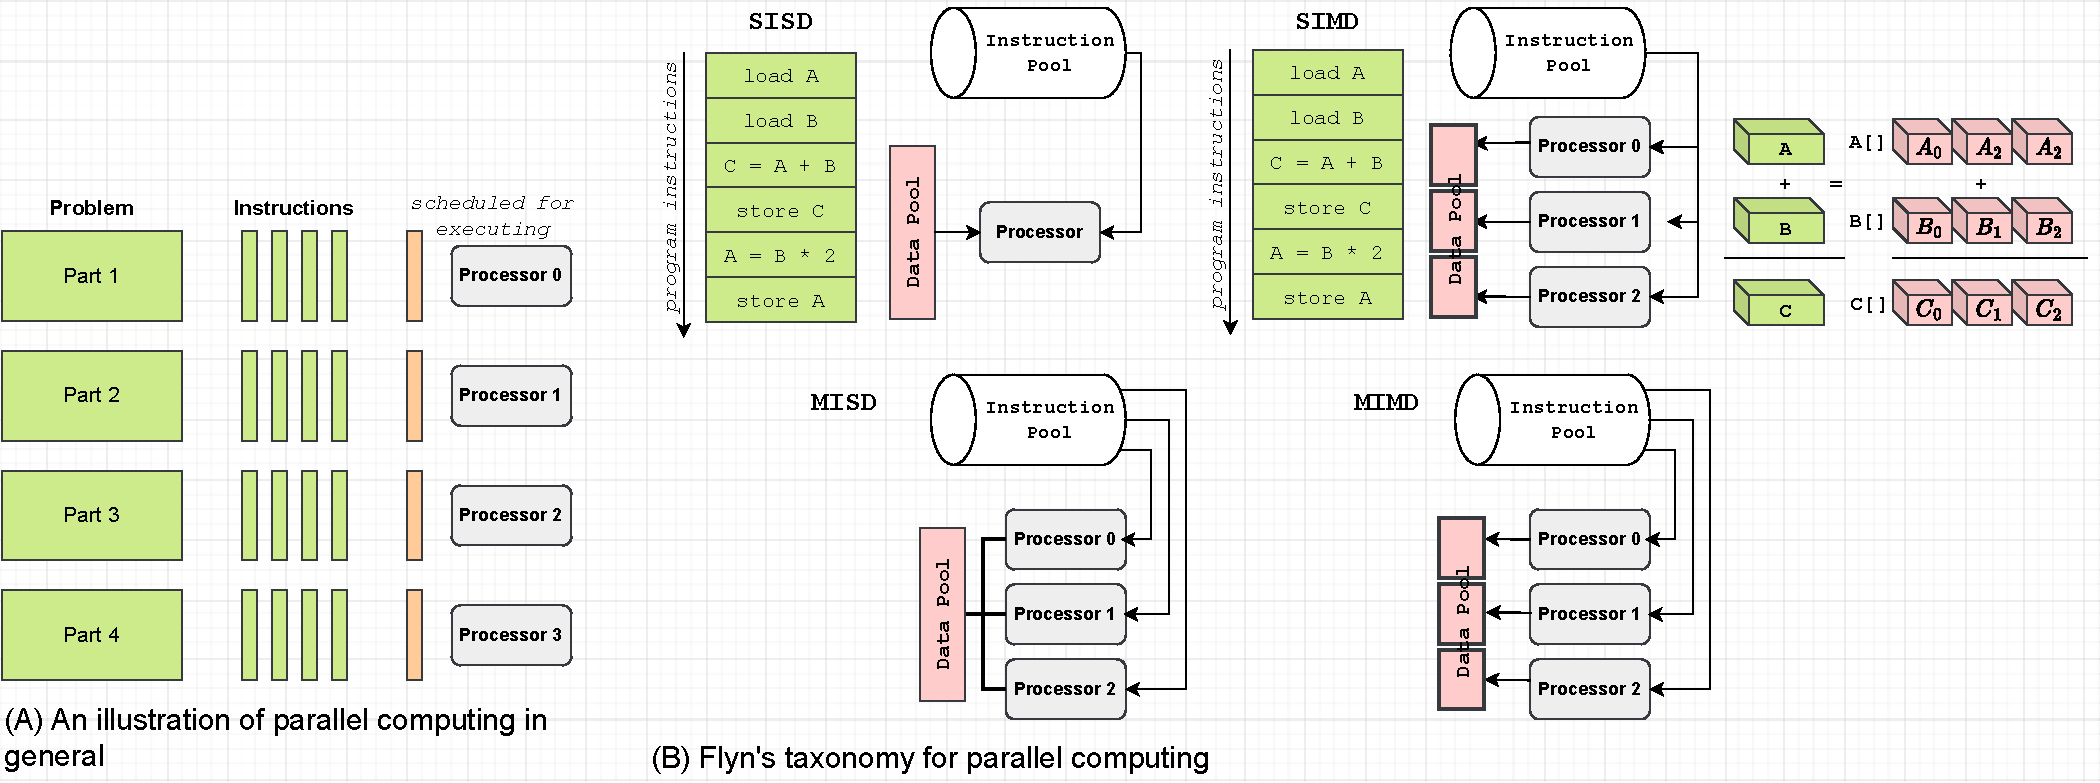
\includegraphics[scale=0.425]{./pictures/preliminaries/preli_parallel_computing_and_taxonomy.pdf}
	\caption{A generic view of parallel computing \cite{hpcllnl2023parcomp}.}
	\label{fig:preli_parallel_computing_and_taxonomy}
\end{figure}

\noindent \textbf{Parallelism}: can happen in different forms, e.g., bit-level parallelism, instruction-level parallelism, data parallelism, and task parallelism \cite{kumar1994intro} \cite{hpcllnl2023parcomp}. Simply put, we assume that a program includes a series of instructions. Sequentially, the program executes one instruction after another, where only one processor is used, and one instruction is executed at once. In parallel, the program can be split into smaller parts running on different processors, where each part now includes a subset of instructions. At the same time, the instructions of different parts can be scheduled to run on different processors. Figure \ref{fig:preli_parallel_computing_and_taxonomy} (A) illustrates an example of parallel computing with four processors. From left to right, we can see the problem divided into four parts, shown as $Part\ 1$, $Part\ 2$, $Part\ 3$, and $Part\ 4$. Each part includes instructions that are scheduled for executing simultaneously on four processors (indexed from $Processor\ 0$ to $Processor\ 3$).\\

Regarding classification, Flynn's taxonomy \cite{kumar1994intro} is widely used. There are four classes shown in Figure \ref{fig:preli_parallel_computing_and_taxonomy} (B), including SISD, SIMD, MISD, and MIMD. Each class is depicted next to its corresponding acronym. The main distinction is based on \textbf{Instruction Stream} and \textbf{Data Stream}, corresponding to the view of von Neumann Computer Architecture \cite{eigenmann1999vonneumanarch}. In detail, each class is characterized as follows.

\begin{itemize}
	\item SISD: Single Instruction Single Data (illustrated in Figure \ref{fig:preli_parallel_computing_and_taxonomy} (B) under the acronym, SISD). Only one instruction is performed, and one data item is manipulated at a time. One arrow stands for an instruction loaded from the instruction pool, and another stands for data manipulation.
	
	\item SIMD: Single Instruction Multiple Data (illustrated in Figure \ref{fig:preli_parallel_computing_and_taxonomy} (B) under the acronym, SIMD). This class of parallel computing has multiple processors, where each processor runs the same instruction on its own data.
	
	\item MISD: Multiple Instruction Single Data (illustrated in Figure \ref{fig:preli_parallel_computing_and_taxonomy} (B) next to the acronym, MISD).
	
	\item MIMD: Multiple Instruction Multiple Data (illustrated in Figure \ref{fig:preli_parallel_computing_and_taxonomy} (B) next to the acronym, MIMD), showing that multiple processors execute multiple instructions and operate multiple data items simultaneously.
\end{itemize}

Expanding from MIMD, some researches divide it into the programming models called Single Program Multiple Data streams (SPMD) \cite{daerma2001spmdmodel} and Multiple Programs Multiple Data streams (MPMD) \cite{fzj2023mpmdmodel}.\\

\begin{figure}[t]
  \centering
  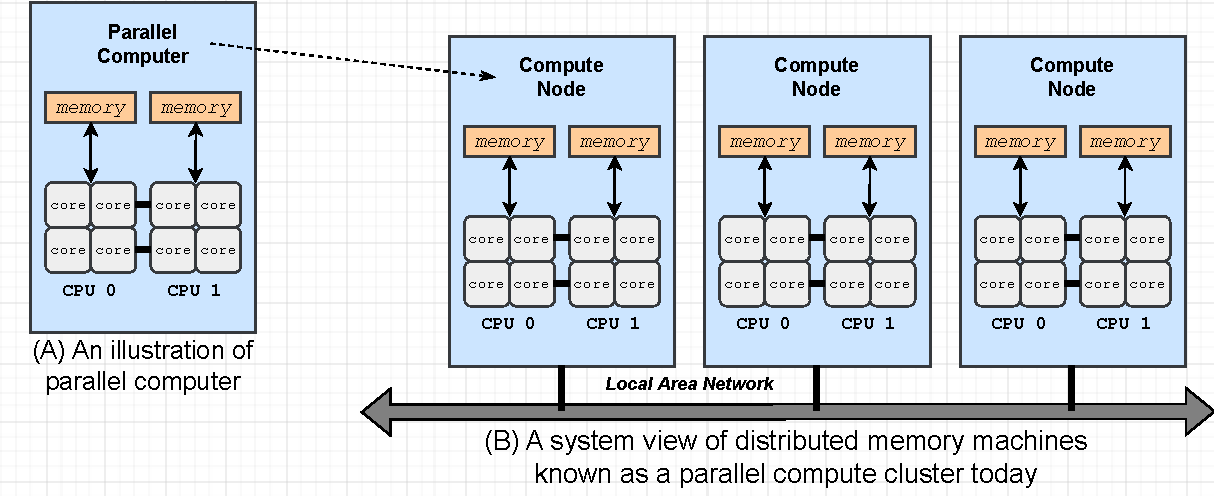
\includegraphics[scale=0.6]{./pictures/preliminaries/preli_parallel_and_distributed_memory_machines.pdf}
	\caption{An example of parallel computers and distributed memory systems know as a parallel compute cluster.}
	\label{fig:preli_parallel_computer_and_cluster}
\end{figure}

\noindent \textbf{Parallel computers:} refers to a computer or a machine with more than one processor (CPU). Sometimes, people imply a CPU as a CPU socket, the physical interface on a motherboard where a CPU is located. In modern computing architectures, a CPU contains multiple cores called single processing units, and each core can execute instructions independently. Each CPU can have its individual memory, where the total memory in a parallel computer is the sum of all individual memories. Figure \ref{fig:preli_parallel_computer_and_cluster} (A) reveals an example of a parallel computer with two CPUs, each with its own memory and containing four cores.\\

Memory access in parallel computers is a complex topic. We can also use the types of memory access to characterize the type of parallel computers. There are mainly two types, shared memory and distributed memory. Shared memory can be noted with all processors accessing the same memory, or a so-called shared address space. Distributed memory can be seen that each CPU has a memory and each refers to a variable on its own memory.\\

From the view of hardware manufactures, the memory architectures of parallel computers are known as
\begin{itemize}
	\item Uniform Memory Access (UMA): all memory locations are accessible to all processors. The access time can be assumed to be identical. A limitation of UMA is the maximum number of processors that can be difficult to expand.
	
	\item Non-Uniform Memory Access (NUMA): each process has a separate memory. This memory architecture can deal with the limit of UMA but leads to a situation where a processor or the cores of a processor access its own memory (local memory) fast and access the other processors' memory (remote memory) slower. Distributed memory implies that a processor cannot directly see another processor's memory. From the programmer's view, there can be a reference to physically and logically distributed memory, which means whether memory is distributed or just appears distributed \cite{victor2010introhpc}. NUMA can be seen as logically and physically distributed, although the distributed nature of NUMA is not apparent to the programmer. Today, most modern computers are made with multicore processors and NUMA architectures.
\end{itemize}

In general, the goal of using parallel computing is to get higher computation performance and access more memory. However, as scientific problems scale up, the complexity of solving them can take a long time to execute on a single computer. Therefore, the idea of parallel compute clusters was built and widely used.\\

\noindent \textbf{Parallel compute clusters:} refers to the architecture used in most supercomputers today. Parallel compute clusters are examples of distributed memory systems. A cluster consists of many computers; in particular, we imply many parallel computers, as explained above. The computers in a cluster are so-called compute nodes. Figure \ref{fig:preli_parallel_computer_and_cluster} (B) demonstrates a parallel compute cluster. All compute nodes can operate as a unified system. Each node connects to another via a local area network (the so-called interconnection network) \cite{baker1999cluster}. The exchange of data or messages between different processors across different nodes is physically distributed memory, where communication overhead might affect the performance of parallel applications. In this thesis, distributed memory indicates the view of memory access in parallel compute clusters. \\

\noindent \textbf{Terminologies}: summarize and emphasize several terminologies based on the explanation above. The following might repeat some notations as well as terms used throughout the thesis.

\begin{itemize}
	\item Cluster: denotes a parallel compute cluster, and is also called an HPC cluster, HPC system, or supercomputer.
	
	\item Node: indicates a compute node in a cluster. Inside a compute node, we have
	\begin{itemize}
		\item Processor or CPU: indicates central processing unit. In computer hardware, a CPU is placed in a CPU socket, which contains mechanical components providing mechanical and electrical connections between a microprocessor and a printed circuit board (PCB). Sometimes, a mentioned CPU socket can also be understood as referring to a CPU.
		\item Core: is single processing unit in a processor. There can be multiple cores inside a processor. Different cores in a node can belong to the same processor or different processors. At the operating system (OS) level, there are
		\begin{itemize}
			\item Process: is an instance of a program. When a process is created and executed, it is defined with its own resources, e.g., memory, file descriptors.
			\item Thread: is an entity within a process. A process can spawn multiple threads inside. While processes are isolated, threads share memory and address space.
		\end{itemize}

		Depending on context switching and mapping algorithm, processes or threads can be mapped dynamically to cores. For performance purposes, a process or thread is often pinned to a specific core in HPC, reducing context switching time. Furthermore, a technology introduced by manufacturer Intel is hyperthreading (Hyper-Threading Technology as HTT or HT) that a single core can run multiple threads. In this case, we call them logical cores in a physical core.
		
	\item Memory: this thesis refers to NUMA architecture in a node (NUMA domain). Each CPU has an individual memory, often called a NUMA node. However, we avoid using NUMA node to ensure no conflict with ``node'' in compute node. We consider the view of memory access in a single node as shared memory. Therefore, it is important to note that
		\begin{itemize}
			\item Shared memory: indicates memory access in a single node.
			\item Distributed memory: indicates memory access across nodes.
		\end{itemize}
	\end{itemize}
	
	\item Communication: implies data or information exchange among processes. These processes can be inside a node or across nodes. To evaluate communication speed, bandwidth is defined as the maximum transmission performance of a network. Generally, bandwidth ($B$) today is measured by megabits, megabytes, or gigabytes per second (Mbps, MBps, or GBps). In HPC networks, communication overhead refers to
	\begin{itemize}
		\item Latency ($\lambda$): the delay time between sending and receiving the header of a message. $\lambda$ can be measured in seconds or milliseconds.
		\item Transmission time or Delay time ($d$): the time for transmitting an entire message between two nodes. Delay ($d$) depends on the size of a message. In the case of no conflict, $d = \lambda + \frac{s}{B}$, where $s$ is the message size. 
	\end{itemize}

\end{itemize}

From the application perspective, users can implement parallel applications using different programming models. The next section introduces general and widespread parallel programming models in common use. Following that, we emphasize our focus on task-based parallel programming models and task-based parallel applications to deal with dynamic load balancing.


% Regarding MPI applications, we might use ranks as an alternative name for processes. Therefore, rank and process can be used interchangeably.
	
%	\item Task: there are different ways to define a task. People may call a task a discrete logical section of computational work. In another context, a task can be a program or a set of instructions executed in sequential or parallel by one or multiple threads/processes. In the thesis's context, we define a parallel program with many tasks.

%	\item Synchronization: denotes the coordination of parallel tasks in real-time. The downsize of synchronization implies waiting for at least one task. Therefore, it can cause a parallel application's wall clock execution time.
%
%	\item Computational Granularity: implies a quantitative or qualitative measure between computation and communication. There are two common terms: \textit{coarse} and \textit{fine}.
%	\begin{itemize}
%		\item Coarse: indicates many computational tasks between communication events.
%		\item Fine: means a small number of computational tasks between communication events.
%	\end{itemize}
%
%	\item Speedup: is a ratio of wallclock execution time between serial execution and parallel execution.
%
%	\item Parallel Overhead: is related to the required execution time, including influence factors such as task start-up time, synchronization, data movement, software overhead, and task termination time.
%
%	\item Scalability: is associated with the ability of a parallel system that can show a proportionate increase in speedup. Several factors, such as hardware, application algorithm, parallel overhead, and application characteristics, can contribute to scalability.

%\textbf{Architectures}: parallel computing systems are mainly designed upon memory models. Almost all machines today revolve around three architectures: shared memory, distributed memory, and hybrid distributed-shared memory.
%\begin{itemize}
%	\item Shared memory machines: is commonly designed with the ability of all processors to access memory like global address space. This architecture has been classified as Uniform Memory Access (UMA) and Non-Uniform Memory Access (NUMA, as mentioned). UMA is  Symmetric Multiprocessor (SMP) with identical processors and equal access time to memory. In contrast, NUMA has a physical link between two or more SMPs. One SMP can access the memory region of another SMP, and they will not have equal access time due to across links.
%	\item Distributed memory machines: often implies a communication overhead via network to link one processor's memory to another. We do not have global address space across all processors because each has its own local memory. Programmers have to define how and when tasks or data are communicated. Importantly, synchronization is essential, and it often belongs to the programmer's responsibility
%	\item Hybrid distributed-shared memory machines: ``hybrid'' refers to the memory model that works on both CPU and graphic processing unit (GPU)/accelerators. There are two main components: shared memory component and distributed memory component. The shared component indicates the connection between CPU and GPU, while the distributed component means the connection between multiple CPU/GPU machines. The current trends show that this computing architecture will be more and more popular in future computing technologies.
%\end{itemize}

%	%---------------------------------
%	\item Distributed memory systems
%	%---------------------------------
%	\begin{itemize}
%		\item Fixed: the number of connections between nodes is fixed. When more processors or nodes are added, they have to share, e.g., Ethernet interconnection.
%		\item Linear: the number of connnections grows linearly when the number of nodes is increased, e.g., mesh-based interconnection.
%		\item Scalable: the number of connections grows as $P\log P$ or even greater, e.g., hypercube interconnection.
%	\end{itemize}
%\end{itemize}

%\input{content/Related-Work}

%\vfill
%\section*{Chapter Summary}
%Chapter~\ref{ch:Motivation} provides the motivation, scopes the problem and derives a requirements' analysis for
%a reference model for \pne management systems for \glspl*{HPC system}.
%Additionally, the related work is presented.
%This presents the problem domain analysis according to the methodical approach of this work (see Sec.~\ref{sec:Intro-Method}).
%
%\begin{figure}[H]%[ht]
%    \centering
%    \resizebox{.98\textwidth}{!}{%
%        \input{pictures/Thesis-Method-Gray/Thesis-Method-Gray2.tikz}
%        }
%        \caption[Method Completion After Chapter 2.]{%
%            Method completion after Chapter 2.}
%            \label{fig:Method-Completion2}
%\end{figure}
